\documentclass[11pt]{scrartcl}

\title{Architektur}
\author{Silvan Adrian \\ Fabian Binna}
\date{\today{}}

\usepackage[ngerman]{babel}
\usepackage[automark]{scrpage2}
\usepackage[colorlinks = true,
linkcolor = black]{hyperref}
\usepackage{color}
\usepackage[normalem]{ulem}
\usepackage{scrpage2}
\usepackage{graphicx}
\usepackage{tabularx}
\graphicspath{ {../22_Grafiken/01_Logo/}{images/}{../../22_Grafiken/01_Logo/} }
\pagestyle{scrheadings}

\clearscrheadfoot
\ihead{
\includegraphics[scale=0.3]{SDDC}}
\ohead{Projekt: SDDC}
\ifoot{Architektur}
\cfoot{Version: 1.00}
\ofoot{Datum: \today{}}
\setheadsepline{0.5pt}
\setfootsepline{0.5pt}

\usepackage{ucs}
\usepackage[utf8]{inputenc}
\usepackage[T1]{fontenc}


\begin{document}
\def\arraystretch{1.5}
\begin{titlepage}
\begin{center}
\vspace{10em}

\includegraphics[scale=2]{SDDC}
\vspace{10em}
\end{center}
\begin{center}
\huge {Architektur}
\end{center}
\begin{center}
\vspace{10em}
\LARGE {Silvan Adrian} \\
\LARGE {Fabian Binna}
\end{center}

\end{titlepage}

\newpage
\section{Änderungshistorie}
\begin{tabularx}{\linewidth}{l l X l}
\textbf{Datum} & \textbf{Version} & \textbf{Änderung}  & \textbf{Autor} \\
\hline
\textbf{17.09.15} & 1.00 & Erstellung des Dokuments & Gruppe \\
\textbf{18.10.2015} & 1.01 & Dokumentaufbau + Logische Sicht & Fabian Binna\\

\end{tabularx}

\newpage
\tableofcontents
\newpage

\subsection{Zweck}
Dieses Dokument beschreibt die Software Architektur für das Projekt SDDC.
\subsection{Gültigkeitsbereich}
Dieses Dokument ist während des ganzen Projekts gültig und wird laufend aktualisiert.

\newpage

\section{Systemübersicht}

\section{Logische Architektur}
Im Package controller wird die REST Schnittstelle implementiert. Die Packages service und orderedservice rufen in der domain die CRUD Methoden auf. Die CRUD Methoden greifen über die dataaccess Schnittstelle auf die generische api und die Datenbank zu. Diese Aufteilung sorgt für einen möglichst modularen Aufbau, ohne unnötige Schichten zu erfinden.

\begin{center}
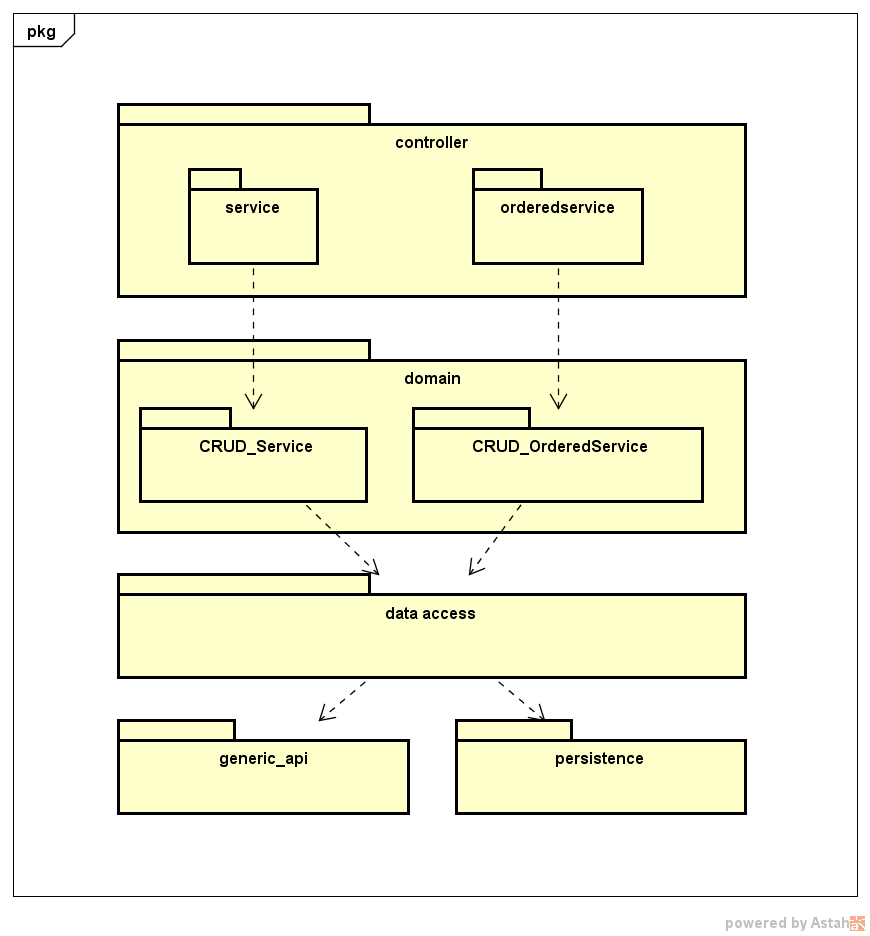
\includegraphics[scale=0.5]{LogischeSicht}
\end{center}

\newpage

\section{Klassenstruktur}

\subsection{controller}
\subsubsection{controller.service}
\subsubsection{controller.orderedservice}

\subsection{domain}
\subsubsection{domain.service}
\subsubsection{domain.orderedservice}

\subsection{data access}
Hier befinden sich die Facaden, welche die Mindestanforderungen für die darunter liegenden Schichten definiert. Das ermöglicht den einfachen Austausch der Implementation für persistence und Infrastruktur (DataCenter).


\subsection{generic api}

\subsection{persistence}

\section{Deployment}

\section{Persistierung}










\end{document}